\documentclass[12pt]{exam}
\usepackage[margin=0.45in]{geometry}
\usepackage[fleqn]{amsmath}
\usepackage{amsfonts,amssymb}
\usepackage{comment,color,soul}
\usepackage{tikz}
\usepackage{hyperref}
\usetikzlibrary{decorations.pathmorphing}

\DeclareMathOperator{\arcsec}{arcsec}
\DeclareMathOperator{\arccot}{arccot}
\DeclareMathOperator{\arccsc}{arccsc}



\newcommand{\ds}{\displaystyle}

\begin{document}
\pagestyle{empty}
\twocolumn
\section*{Formula Sheet} 
\footnotesize

\noindent
\textbf{Quadratic Formula}  
$$\ds x = \frac{-b \pm \sqrt{b^2 - 4ac}}{2a}$$

\noindent
\textbf{Point-Slope Form}
$$y-y_1 = m(x-x_1)$$

\noindent
\textbf{Common Angles} \\
\noindent
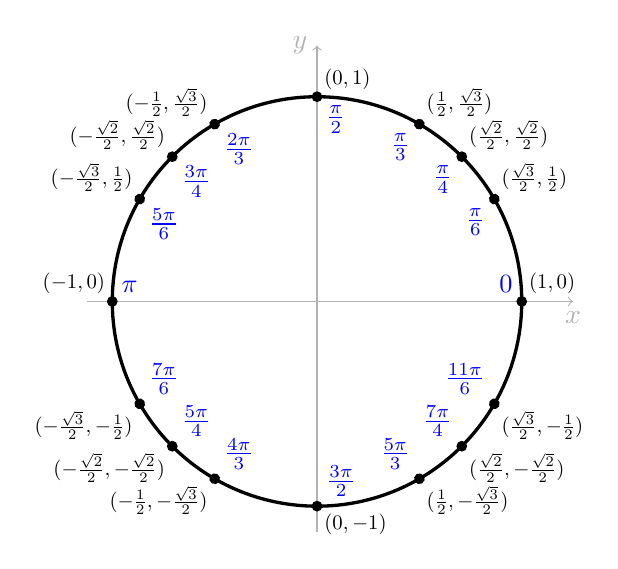
\begin{tikzpicture}[scale=0.65]
\draw[color=black!30,->] (0,-4.5) -- (0,5) node[left] {$y$};
\draw[color=black!30,->] (-4.5,0) -- (5,0) node[below] {$x$};
\draw[very thick] (0,0) circle (4); 
% The x,y-coordinates are given in black.  
\foreach \angle/\coordinates/\position in {
% 1st Quadrant
30/{$(\frac{\sqrt{3}}{2},\frac{1}{2})$}/{above right},45/{$(\frac{\sqrt{2}}{2},\frac{\sqrt{2}}{2})$}/{above right},60/{$(\frac{1}{2},\frac{\sqrt{3}}{2})$}/{above right},
%Four Corners
0/{$(1,0)$}/{above right},90/{$(0,1)$}/{above right},180/{$(-1,0)$}/{above left},270/{$(0,-1)$}/{below right},
% 2nd Quadrant
120/{$(-\frac{1}{2},\frac{\sqrt{3}}{2})$}/{above left},135/{$(-\frac{\sqrt{2}}{2},\frac{\sqrt{2}}{2})$}/{above left},150/{$(-\frac{\sqrt{3}}{2},\frac{1}{2})$}/{above left}, 
% 3rd Quadrant
210/{$(-\frac{\sqrt{3}}{2},-\frac{1}{2})$}/{below left},225/{$(-\frac{\sqrt{2}}{2},-\frac{\sqrt{2}}{2})$}/{below left},240/{$(-\frac{1}{2},-\frac{\sqrt{3}}{2})$}/{below left},
% 4th Quadrant
300/{$(\frac{1}{2},-\frac{\sqrt{3}}{2})$}/{below right},315/{$(\frac{\sqrt{2}}{2},-\frac{\sqrt{2}}{2})$}/{below right},330/{$(\frac{\sqrt{3}}{2},-\frac{1}{2})$}/{below right}} 
{
\fill[rotate=\angle] (4,0) circle (3pt);
\draw[rotate=\angle] (4,0) node[scale=0.75,\position] {\coordinates};
}
% The radians increments are given in blue.
\foreach \angle/\radians/\position in {
% 1st Quadrant
30/{$\frac{\pi}{6}$}/{below left},45/{$\frac{\pi}{4}$}/{below left},60/{$\frac{\pi}{3}$}/{below left},
%Four Corners
0/{$0$}/{above left},90/{$\frac{\pi}{2}$}/{below right},180/{$\pi$}/{above right},270/{$\frac{3\pi}{2}$}/{above right},
% 2nd Quadrant
120/{$\frac{2\pi}{3}$}/{below right},135/{$\frac{3\pi}{4}$}/{below right},150/{$\frac{5\pi}{6}$}/{below right}, 
% 3rd Quadrant
210/{$\frac{7\pi}{6}$}/{above right},225/{$\frac{5\pi}{4}$}/{above right},240/{$\frac{4\pi}{3}$}/{above right},
% 4th Quadrant
300/{$\frac{5\pi}{3}$}/{above left},315/{$\frac{7 \pi}{4}$}/{above left},330/{$\frac{11 \pi}{6}$}/{above left}} 
{
\draw[color=blue,rotate=\angle] (4,0) node[scale=0.95,\position] {\radians};
}
\end{tikzpicture}


\noindent
\textbf{Trigonometry Ratios} ~
\begin{itemize}
\item $\ds \tan x = \frac{\sin x}{\cos x} ~~~~ \ds \cot x = \frac{\cos x}{\sin x}$
\bigskip

\item $\ds \sec x = \frac{1}{\cos x} ~~~~ \ds \csc x =  \frac{1}{\sin x}$
\bigskip
\end{itemize}

\noindent 
\textbf{Angle Addition Identities} ~
\begin{itemize}
\item $\cos(a+b) = \cos a \cos b - \sin a \sin b$
\bigskip

\item $\sin(a+b) = \sin a \cos b + \sin b \cos a$
\bigskip
\end{itemize}

\noindent
\textbf{Trigonometry Limits} ~
\begin{itemize}
\item $\ds \lim_{x \rightarrow 0} \frac{\sin x}{x} = 1$
\bigskip

\item $\ds \lim_{x \rightarrow 0} \frac{1-\cos x}{x} =0$
\bigskip
\end{itemize}

\noindent
\textbf{Definition of Derivative} ~
\begin{itemize}
\item $\ds f'(x) = \lim_{h\rightarrow 0} \frac{f(x+h)-f(x)}{h}$, or 
\bigskip

\item $\ds f'(a) = \lim_{x\rightarrow a} \frac{f(x)-f(a)}{x-a}$
\bigskip
\end{itemize}


\newpage

\noindent
\textbf{Selected Derivatives} ~ 
\begin{itemize}
\item $\ds \frac{d}{dx} \tan x = \sec^2 x $
\bigskip

\item $\ds \frac{d}{dx} \sec x = \sec x \tan x$
\bigskip

\item $\ds \frac{d}{dx} \cot x = -\csc^2 x $
\bigskip
\item $\ds \frac{d}{dx} \csc x = -\csc x \cot x$
\bigskip
\end{itemize}


\noindent
\textbf{Linear Approximation} ~
\begin{itemize}
\item $\ds f(x) \approx f(a) + f'(a)(x-a)$
\bigskip
\end{itemize}



\noindent
\textbf{Error and Relative Error} ~
\begin{itemize}
\item $dy \approx$ the error in $y$
\bigskip
\item $\dfrac{dy}{y} \approx$ the relative (percent) error in $y$
\bigskip
\end{itemize}

\noindent
\textbf{Newton's Method} ~
\begin{itemize}
\item $\ds x_{n+1} = x_n - \frac{f(x_n)}{f'(x_n)}$
\bigskip
\end{itemize}

\noindent
\textbf{Summation Formulas} ~
\begin{itemize}
\item $\ds \sum_{i = 1}^n i = \frac{n(n+1)}{2}$
\item $\ds \sum_{i = 1}^n i^2 = \frac{n(n+1)(2n+1)}{6}$
\bigskip
\end{itemize}

\noindent
\textbf{Riemann Sum} ~
\begin{itemize}
\item $\ds A \approx \sum_{i = 1}^n f(x_i) \Delta x$ where
\item $\ds \Delta x = \frac{b-a}{n}$ and 
\item $\ds x_i = a + i \Delta x$
\bigskip
\end{itemize}

\noindent
\textbf{Average Value of a Function} ~
\begin{itemize}
\item $\ds \frac{1}{b-a}\int_a^b f(x) \, dx$
\bigskip
\end{itemize}



\end{document}


\end{document}
